

\section{Entorno de Simulación}

Para lograr este objetivo, se optó por desarrollar un entorno de simulación robusto y versátil utilizando el motor de videojuegos Unreal Engine 5. La elección de Unreal Engine 5 se fundamenta en varias de sus características clave que se alinean directamente con las necesidades del proyecto:

\begin{itemize}
    \item \textbf{Realismo Visual y Físico:} Unreal Engine 5 ofrece capacidades gráficas de vanguardia y un motor de físicas avanzado. Esto permite recrear escenarios de operación con un alto grado de fidelidad, lo que es crucial para validar algoritmos de visión computacional y la interacción del robot con el entorno. Se pueden simular diversas condiciones de iluminación, terrenos y obstáculos que el robot podría encontrar en un despliegue real.
    \item \textbf{Flexibilidad y Extensibilidad:} El motor proporciona un amplio conjunto de herramientas y la posibilidad de C++ scripting, lo que permite una personalización profunda del entorno de simulación. Esto facilita la integración de modelos específicos del robot, sensores (como cámaras, LiDAR) y actuadores, así como la implementación de lógicas de comportamiento complejas para los objetivos y otros agentes en el simulador.
    \item \textbf{Generación de Datos Sintéticos:} Una ventaja significativa es la capacidad de generar grandes volúmenes de datos sintéticos etiquetados. Estos datos son invaluables para el entrenamiento y la validación de los modelos de aprendizaje automático utilizados en el sistema de identificación de objetivos, reduciendo la dependencia de la recolección de datos en el mundo real, que puede ser costosa y peligrosa en un contexto militar.
    \item \textbf{Iteración Rápida:} La naturaleza interactiva de un motor de videojuegos permite realizar pruebas y ajustes de manera ágil. Se pueden modificar parámetros del robot, del entorno o de la misión y observar los resultados de forma inmediata, acelerando el ciclo de desarrollo y depuración.
    \item \textbf{Soporte Comunitario y Documentación:} Unreal Engine cuenta con una vasta comunidad de desarrolladores y una extensa documentación, lo que facilita la resolución de problemas y el aprendizaje de funcionalidades avanzadas.
\end{itemize}

El simulador desarrollado permite configurar diferentes escenarios de misión, variando elementos como la disposición de los objetivos, las características del terreno, la presencia de obstáculos y las condiciones ambientales. Esto no solo sirve para probar la robustez general del sistema de navegación y control del robot, sino también para evaluar la efectividad de las estrategias de identificación y eliminación de objetivos bajo diversas circunstancias.

\begin{figure}[htbp]
\centering
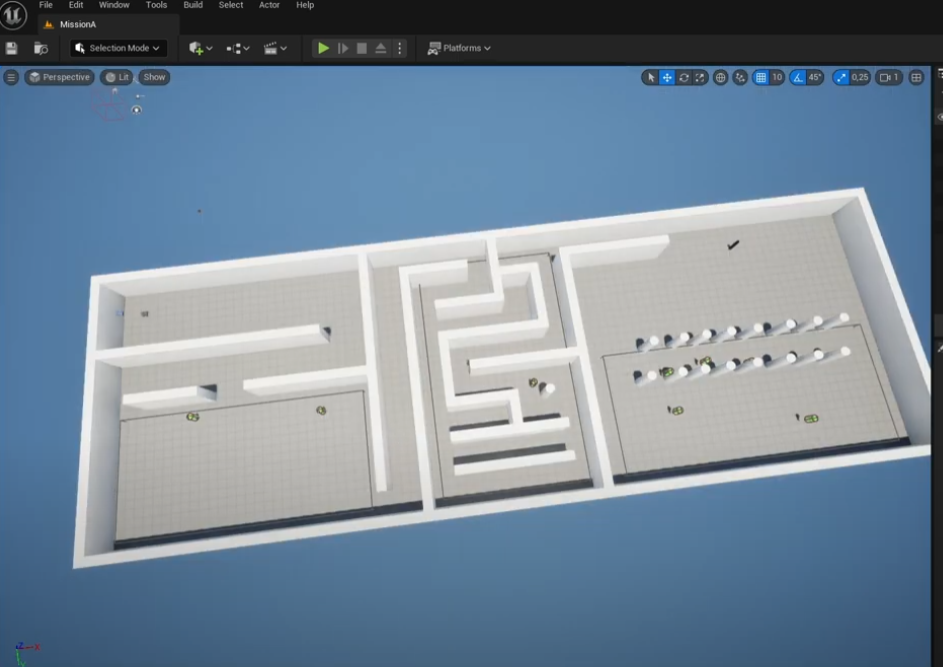
\includegraphics[width=.75\textwidth]{Figures/UE5.png}
\caption{Captura del entorno de simulación en Unreal Engine 5.}
\label{fig:simulador_entorno}
\end{figure}
%TODO agregar mas imagenes

En resumen, la utilización de Unreal Engine 5 como base para el simulador ha proporcionado una plataforma potente y adaptable, esencial para el desarrollo, prueba y validación iterativa del sistema robótico militar propuesto en esta tesis. Permite emular con precisión las condiciones operativas y evaluar el desempeño de los algoritmos de visión computacional y aprendizaje automático en un entorno seguro y controlado antes de su implementación en el prototipo físico.